\documentclass[11pt]{article}
\usepackage{amsmath}
\usepackage{amssymb}
\usepackage{tikz}
\usetikzlibrary{arrows.meta, angles, quotes}

\begin{document}

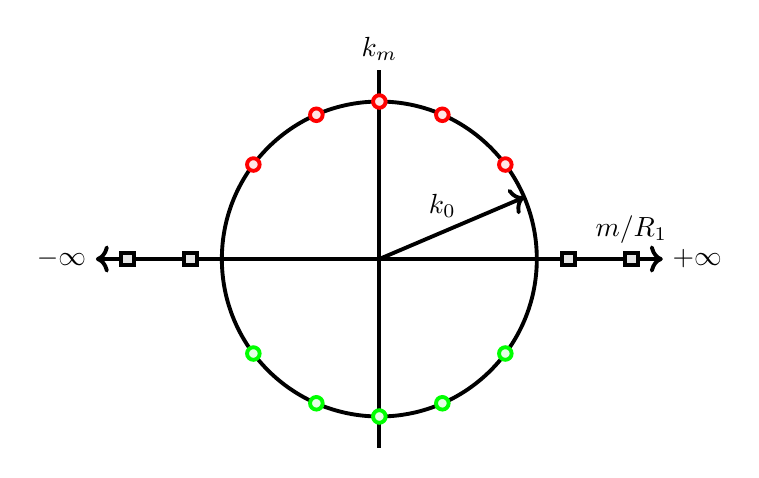
\begin{tikzpicture}[scale=0.8]
\draw [black,line width=1.4] (4,3) circle (2.5);
\draw [line width=1.4, <->] (-0.5,3) -- (8.5,3);
\draw [line width=1.4] (4,0) -- (4,6);

\draw [line width=1.4,->] (4,3) -- (6.3,3.98);

\draw [red,line width=1.4,fill=red!10] (4,5.5) circle (0.1);
\draw [red,line width=1.4,fill=red!10] (5,5.29) circle (0.1);
\draw [red,line width=1.4,fill=red!10] (6,4.5) circle (0.1);

\draw [red,line width=1.4,fill=red!10] (3,5.29) circle (0.1);
\draw [red,line width=1.4,fill=red!10] (2,4.5) circle (0.1);

\draw [green,line width=1.4,fill=green!10] (4,0.5) circle (0.1);
\draw [green,line width=1.4,fill=green!10] (5,0.71) circle (0.1);
\draw [green,line width=1.4,fill=green!10] (6,1.5) circle (0.1);

\draw [green,line width=1.4,fill=green!10] (3,0.71) circle (0.1);
\draw [green,line width=1.4,fill=green!10] (2,1.5) circle (0.1);

\draw [black,line width=1.4,fill=black!10] (-0.1,2.9) rectangle (0.1,3.1);
\draw [black,line width=1.4,fill=black!10] (0.9,2.9) rectangle (1.1,3.1);
\draw [black,line width=1.4,fill=black!10] (6.9,2.9) rectangle (7.1,3.1);
\draw [black,line width=1.4,fill=black!10] (7.9,2.9) rectangle (8.1,3.1);

\node at (5,3.5) [anchor=south]{$k_0$};
\node at (8,3.1) [anchor=south]{$m /R_1$};
\node at (4,6) [anchor=south]{$k_m$};
\node at (-0.5,3) [anchor=east]{$-\infty$};
\node at (8.5,3) [anchor=west]{$+\infty$};

\end{tikzpicture}

\end{document}